\section{Phân tích Tổng quan các Hệ thống Liên quan trên Thị trường}

\subsection{Hệ thống Quản lý và Tra cứu Tài nguyên Thư viện -- Trường Đại học Bách Khoa - ĐHQG TP.HCM (HCMUT)}

Hệ thống quản lý và tra cứu tài nguyên thư viện tại Trường Đại học Bách Khoa (ĐHQG TP.HCM) hiện đang vận hành thông qua hai cổng thành phần độc lập nhưng bổ trợ lẫn nhau: Cổng Thông tin Thư viện Chính thức (\url{https://lib.hcmut.edu.vn/}) và hệ thống Tra cứu Danh mục Công cộng Trực tuyến (OPAC tại \url{https://opac.lib.hcmut.edu.vn/}). Sự kết hợp này nhằm quản lý và phục vụ song song hai luồng tài nguyên cốt lõi: tài liệu in truyền thống và các tài sản lưu trữ thuộc sở hữu của nhà trường.

Đối với cổng thông tin thư viện chính (\url{lib.hcmut.edu.vn}), hệ thống đóng vai trò như một trung tâm tập trung quản lý và hiển thị toàn bộ tài liệu in, bao gồm giáo trình, sách tham khảo và các tạp chí khoa học thuộc nhiều chuyên ngành được lưu trữ vật lý tại các kho sách trong cơ sở (như Bộ sưu tập Mượn tại Nhà B2, Bộ sưu tập Tham khảo tại Nhà B4 Cơ sở Lý Thường Kiệt, và Thư viện tại Cơ sở Dĩ An). Người dùng trên giao diện này chủ yếu truy cập các thông báo chung, quy định mượn trả, hoặc sử dụng thanh tìm kiếm nhanh để xác minh sự sẵn có vật lý của các tập sách in.

\begin{figure}[H]
    \centering
     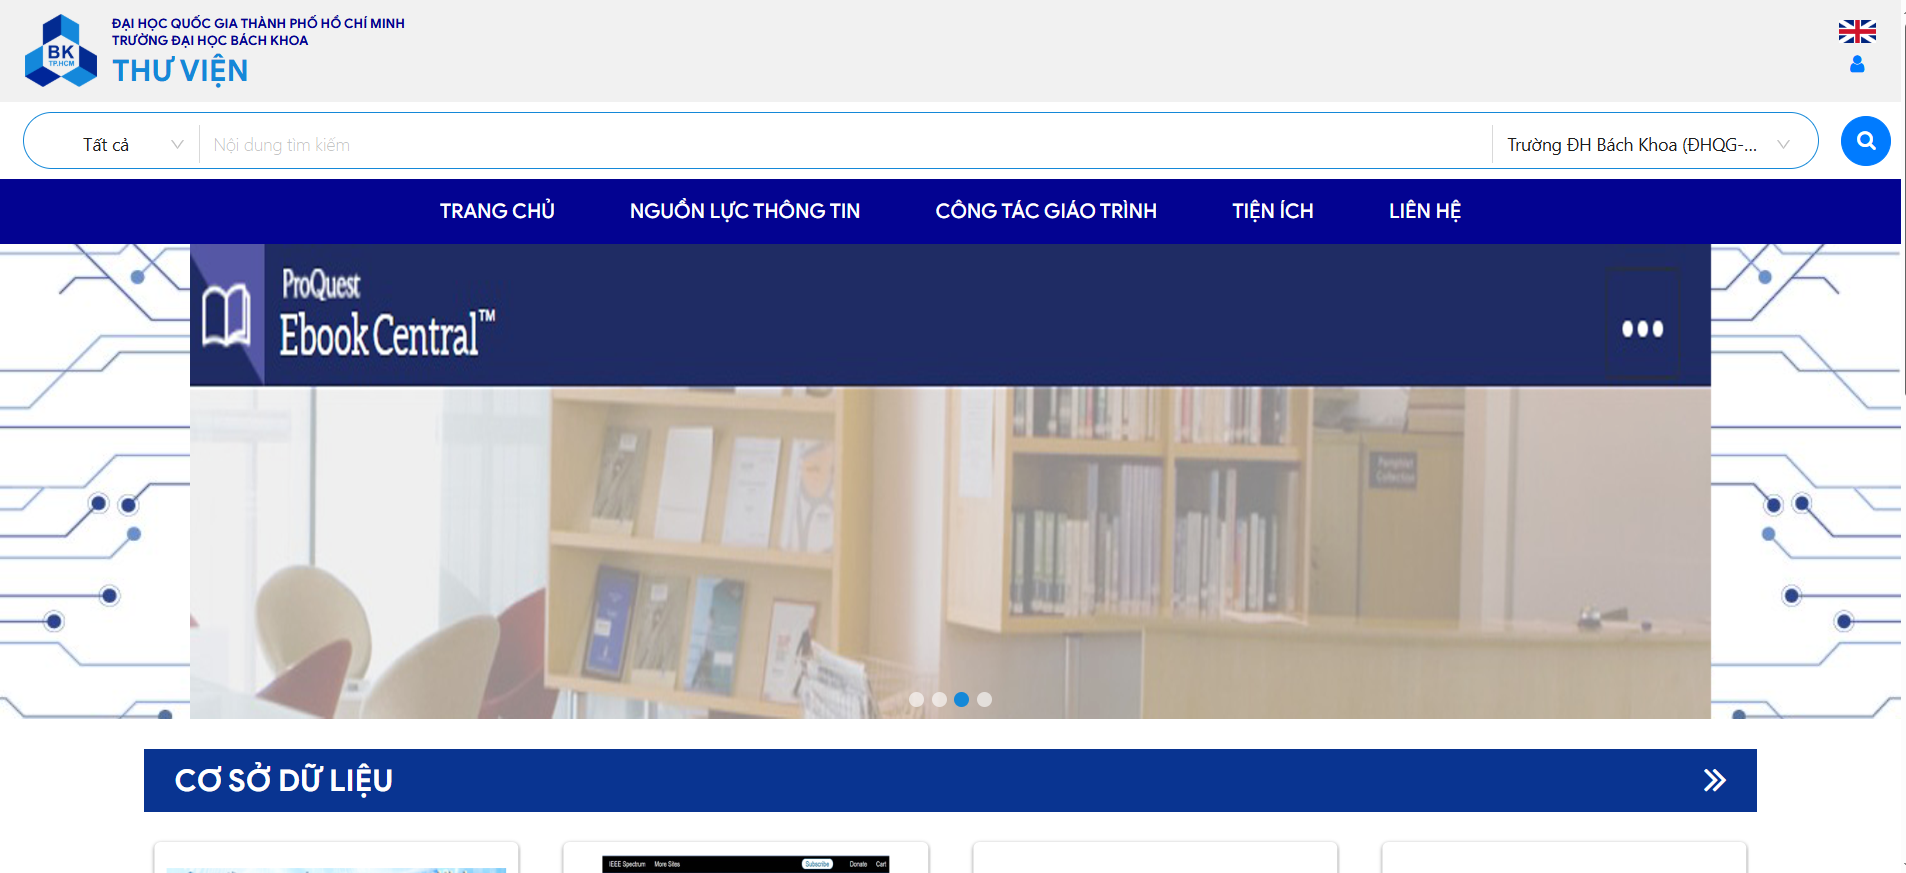
\includegraphics[width=0.8\linewidth]{Images/lib_hcmut_homepage.png} 
     \vspace{10pt}
    \caption{Giao diện chính cổng thông tin thư viện lib.hcmut.edu.vn và danh mục tài liệu in}
    \label{fig:lib_hcmut_homepage}
\end{figure}

Đồng thời, để hỗ trợ nghiên cứu khoa học chuyên sâu, nhà trường vận hành cổng OPAC (\url{opac.lib.hcmut.edu.vn}), đóng vai trò là cổng tra cứu chuyên biệt cho các tài sản lưu trữ của trường. Cổng này lưu trữ và số hóa các tài sản trí tuệ được sản xuất trong nhà trường, bao gồm khóa luận tốt nghiệp của sinh viên, luận văn cao học, luận án tiến sĩ và các đề tài nghiên cứu khoa học của giảng viên. Giao diện OPAC cung cấp bộ lọc dữ liệu tả nâng cao theo Tác giả, Người hướng dẫn, Năm bảo vệ hoặc Lĩnh vực chuyên môn.

Hệ thống OPAC được tích hợp sâu với hệ thống xác thực Đăng nhập Một lần (SSO/BKPay) của nhà trường. Sau khi đăng nhập thành công vào mô-đun "Tài khoản Cá nhân", độc giả có thể quản lý các hoạt động mượn sách như xem các mục đang mượn, kiểm tra lịch sử mượn, theo dõi tiền phạt quá hạn, yêu cầu gia hạn mượn, hoặc đặt chỗ cho các tài liệu hiện đang được mượn hết.

\begin{figure}[H]
    \centering
    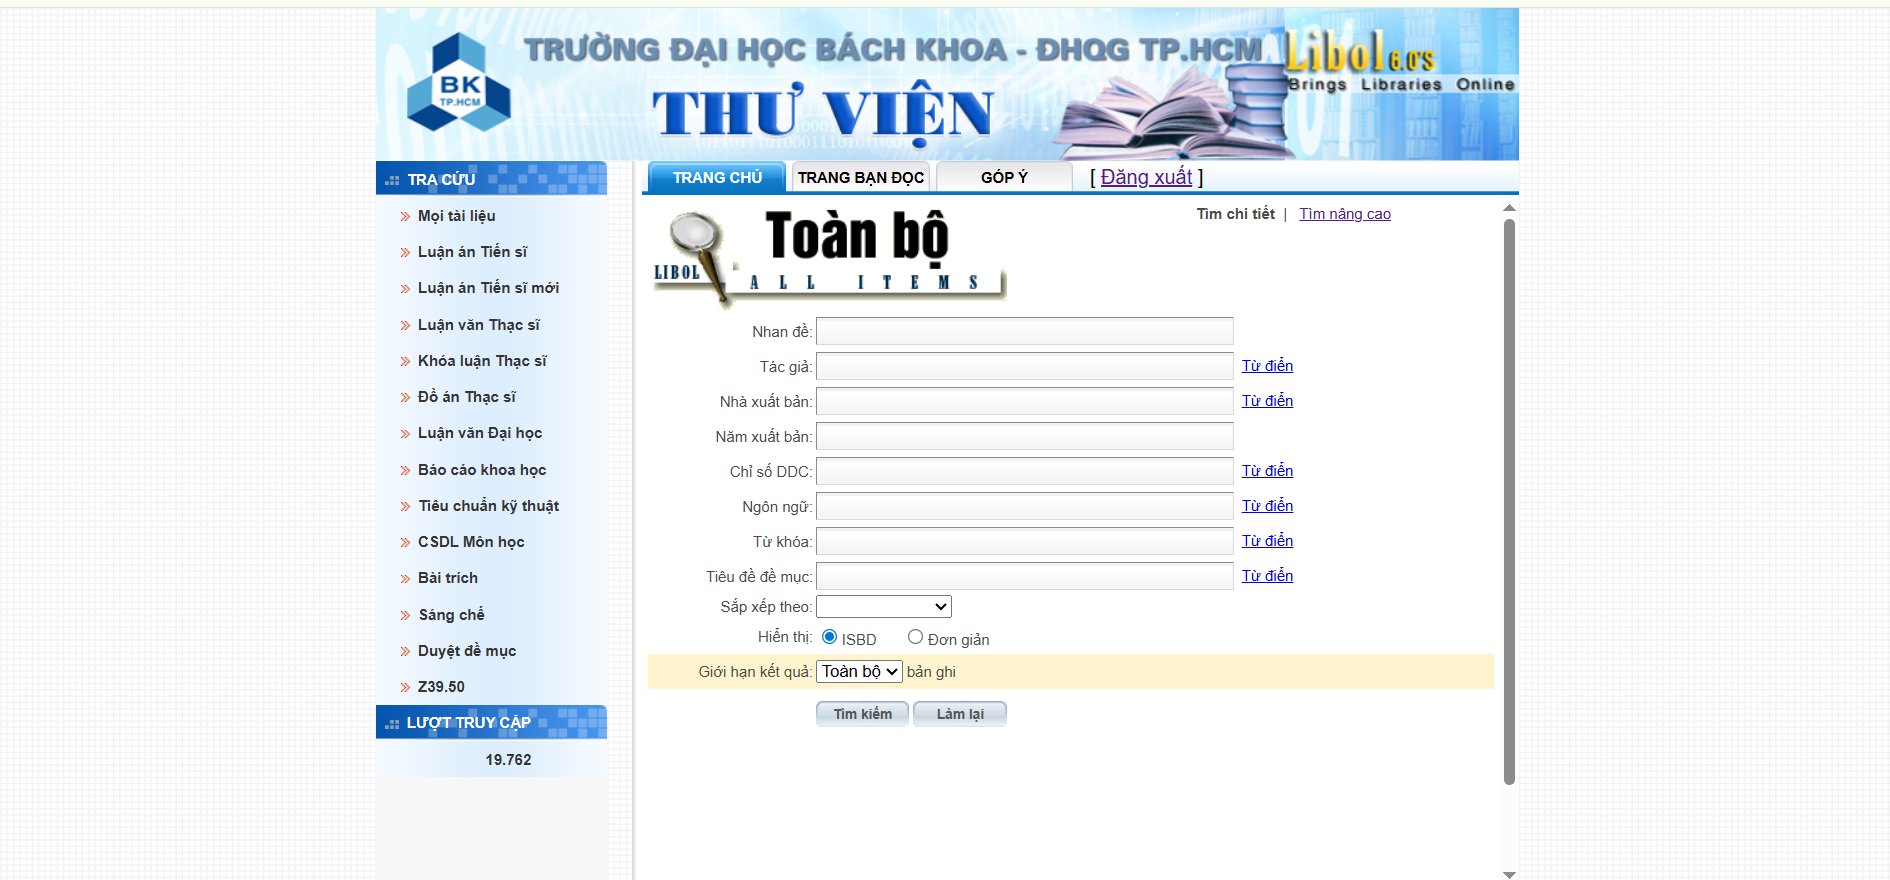
\includegraphics[width=0.8\linewidth]{Images/opac.lib.hcmut.edu.vn.png} 
     \vspace{10pt}
    \caption{Giao diện Tra cứu Tài liệu Lưu trữ Nội bộ và Mô-đun Đăng nhập Tài khoản trên cổng OPAC}
    \label{fig:opac_hcmut_search}
\end{figure}

Mặc dù cả hai cổng đều đáp ứng các nhu cầu vận hành cốt lõi, việc phân mảnh dữ liệu giữa tài liệu in và kho tài liệu số/lưu trữ nội bộ tạo ra sự bất tiện trong trải nghiệm của sinh viên. Hạn chế này là động lực để nhóm chúng tôi xây dựng một hệ thống quản lý thư viện hiện đại giúp hợp nhất dữ liệu tài nguyên và tối ưu hóa quy trình vận hành thông qua các giải pháp phần mềm hiện đại.

\subsubsection{Ưu điểm}
\begin{itemize}
    \item Giao diện chuyên biệt cho tài liệu lưu trữ nội bộ được tối ưu hóa để truy vấn các trường dữ liệu tả học thuật.
    \item Quy trình mượn-trả trực tuyến và đặt giữ chỗ hoàn toàn tương thích với các chính sách thư viện thực tế.
    \item Cơ chế xác thực Đăng nhập Một lần (SSO) đồng bộ tài khoản độc giả đồng thời bảo mật tài nguyên số.
\end{itemize}

\subsubsection{Hạn chế}
\begin{itemize}
    \item Việc duy trì hai cổng độc lập buộc độc giả phải thực hiện các thao tác tìm kiếm lặp đi lặp lại trên các tên miền riêng biệt.
    \item Cơ chế tìm kiếm dựa hoàn toàn vào khớp từ khóa chính xác, khả năng hiểu ngôn ngữ tự nhiên còn hạn chế.
    \item Kiến trúc nền tảng tĩnh thiếu các tính năng gợi ý tự động và công cụ trợ lý ảo AI 24/7.
    \item Giao diện tìm kiếm nâng cao chưa được tối ưu tốt cho các thiết bị di động, quy trình tương tác còn mang tính thủ tục.
\end{itemize}

\subsection{Hệ thống Thư viện Trực tuyến -- Đại học London (The Online Library -- UoL)}

Hệ thống Thư viện Trực tuyến của Đại học London (UoL) tại \url{https://onlinelibrary.london.ac.uk/} đại diện cho mô hình thư viện số (E-library) hàng đầu được thiết kế chuyên biệt để hỗ trợ sinh viên học từ xa trên toàn cầu. Khác với các mô hình quản lý bộ sưu tập vật lý truyền thống, hệ thống này vận hành hoàn toàn trên môi trường số, tập trung vào việc quản lý, lưu trữ và phân phối quyền truy cập vào các cơ sở dữ liệu học thuật, tạp chí điện tử (E-journals) và sách điện tử (E-books).

Điểm sáng kỹ thuật của hệ thống là việc triển khai Dịch vụ Khám phá Tập trung (Discovery Service). Thay vì yêu cầu người dùng đăng nhập vào từng nền tảng của nhà xuất bản, một thanh tìm kiếm hợp nhất (One-stop search) có thể truy vấn các mục toàn văn trên hàng trăm nguồn cơ sở dữ liệu. Hơn nữa, để bù đắp cho sự thiếu hụt hỗ trợ trực tiếp tại chỗ, hệ thống cung cấp công cụ hỗ trợ trực tuyến ("Chat với chúng tôi") hoạt động như một bàn trợ giúp 24/7 để giải quyết các thắc mắc kỹ thuật và hướng dẫn sinh viên tìm kiếm tài liệu.

\begin{figure}[H]
    \centering
     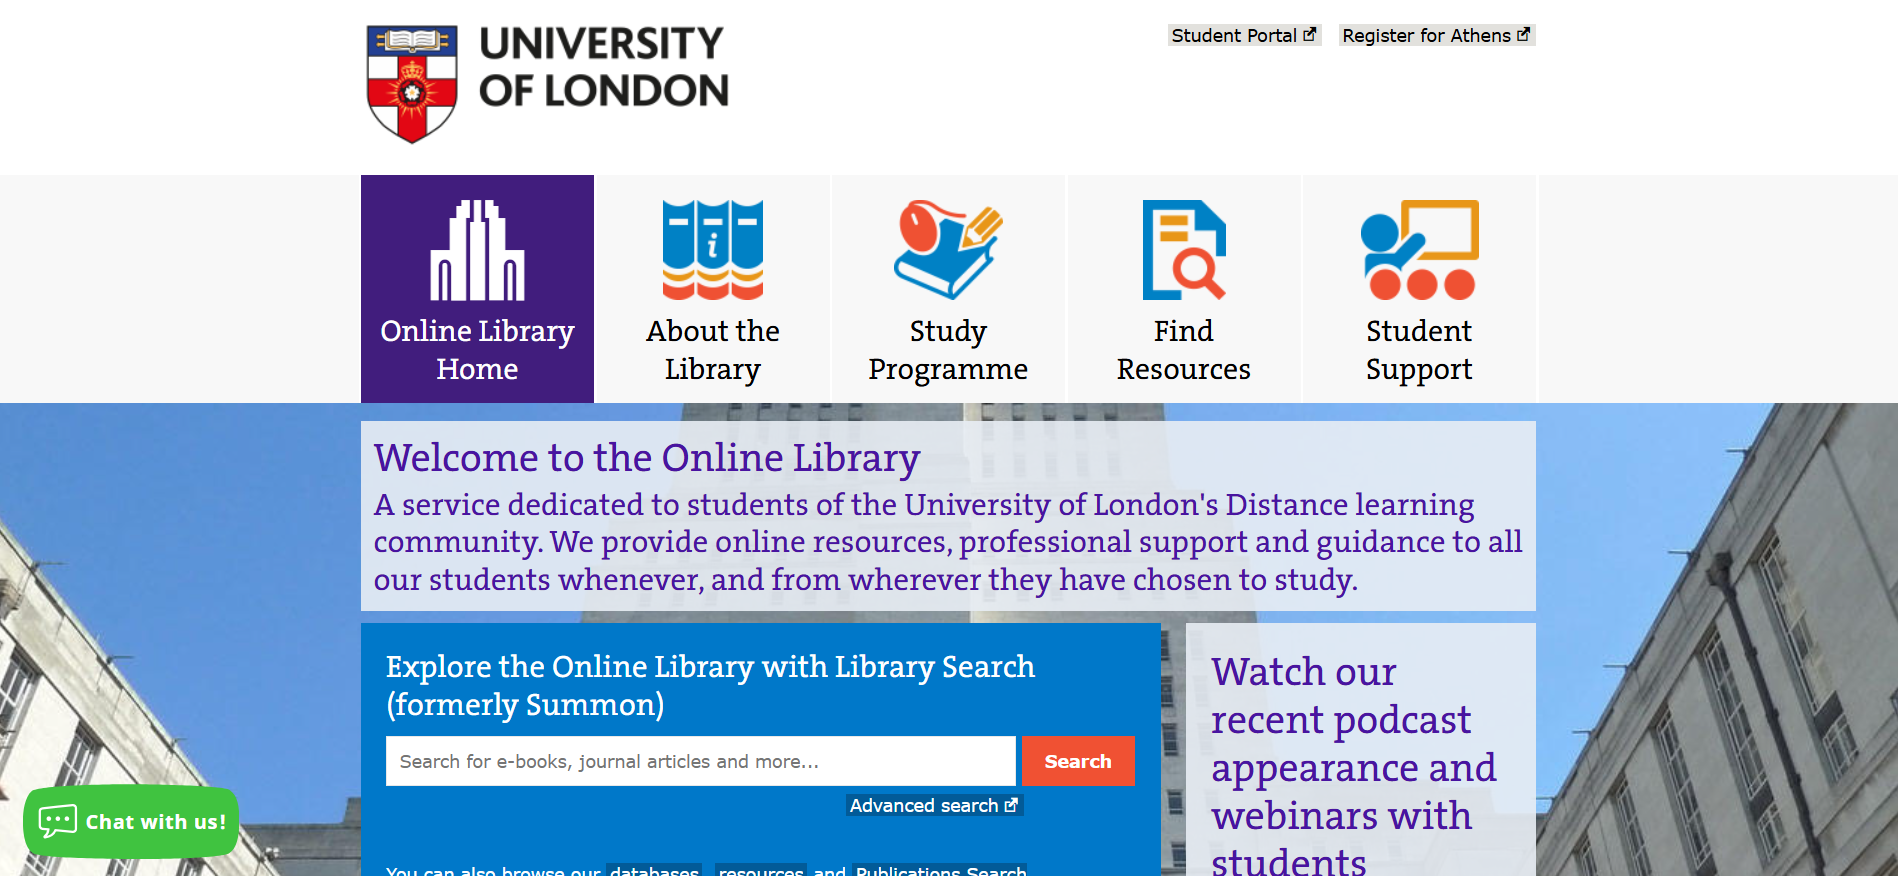
\includegraphics[width=0.8\linewidth]{Images/london_online_library_homepage.png} 
    \vspace{10pt}
    \caption{Giao diện tìm kiếm khám phá hợp nhất và công cụ hỗ trợ trực tuyến tại Thư viện Trực tuyến UoL}
    \label{fig:london_lib_homepage}
\end{figure}

Phân tích hệ thống của UoL mang lại những góc nhìn quan trọng về việc tối ưu hóa trải nghiệm người dùng số, đồng thời làm nổi bật các khoảng trống công nghệ trong việc tương tác thông minh với người dùng.

\subsubsection{Ưu điểm}
\begin{itemize}
    \item Cung cấp một cổng truy cập duy nhất cho tất cả các tài nguyên số, giảm thời gian tìm kiếm cho người dùng.
    \item Sử dụng các giao thức xác thực hiện đại (OpenAthens), cho phép truy cập từ xa ngoài khuôn viên trường một cách mượt mà mà không cần VPN.
    \item Phân loại tài liệu số theo các ngành học cụ thể để hướng dẫn sinh viên khám phá tài liệu hiệu quả.
\end{itemize}

\subsubsection{Hạn chế}
\begin{itemize}
    \item Mô hình chỉ giới hạn trong các tài sản số, bỏ qua hoàn toàn quy trình lưu thông sách vật lý và quản lý kho sách.
    \item Việc tìm kiếm khám phá tập trung có thể gây ra tình trạng quá tải thông tin và thiếu phân tích hành vi để gợi ý cá nhân hóa.
    \item Hỗ trợ chatbot hoạt động dựa trên các quy tắc kịch bản tĩnh, chưa thể hiểu các câu truy vấn phức tạp và phụ thuộc nhiều vào sự can thiệp của thủ thư.
\end{itemize}

\subsection{Hệ thống Thư viện Đại học Delaware (UD Library)}

Hệ thống Thư viện Đại học Delaware (UD Library) tại \url{https://library.udel.edu/} là minh họa cho mô hình quản trị thư viện đại học đa chi nhánh được số hóa cao. Khác với định hướng thuần số của UoL, UD Library giải quyết một bài toán phức tạp hơn: quản lý và phân phối dữ liệu giữa thư viện trung tâm và các thư viện khoa, đồng thời tiên phong tích hợp trợ lý ảo AI vào quy trình hỗ trợ sinh viên.

Cốt lõi của hệ thống này là \textbf{DELCAT} (Dịch vụ Khám phá Hợp nhất), đóng vai trò là giao diện duy nhất kết nối người dùng với hàng triệu bản ghi thuộc nhiều định dạng khác nhau. Đáng chú ý, UD Library đã bắt đầu triển khai các giải pháp AI giao tiếp bằng ngôn ngữ tự nhiên bên cạnh các cơ chế tìm kiếm truyền thống.

\begin{figure}[H]
\centering
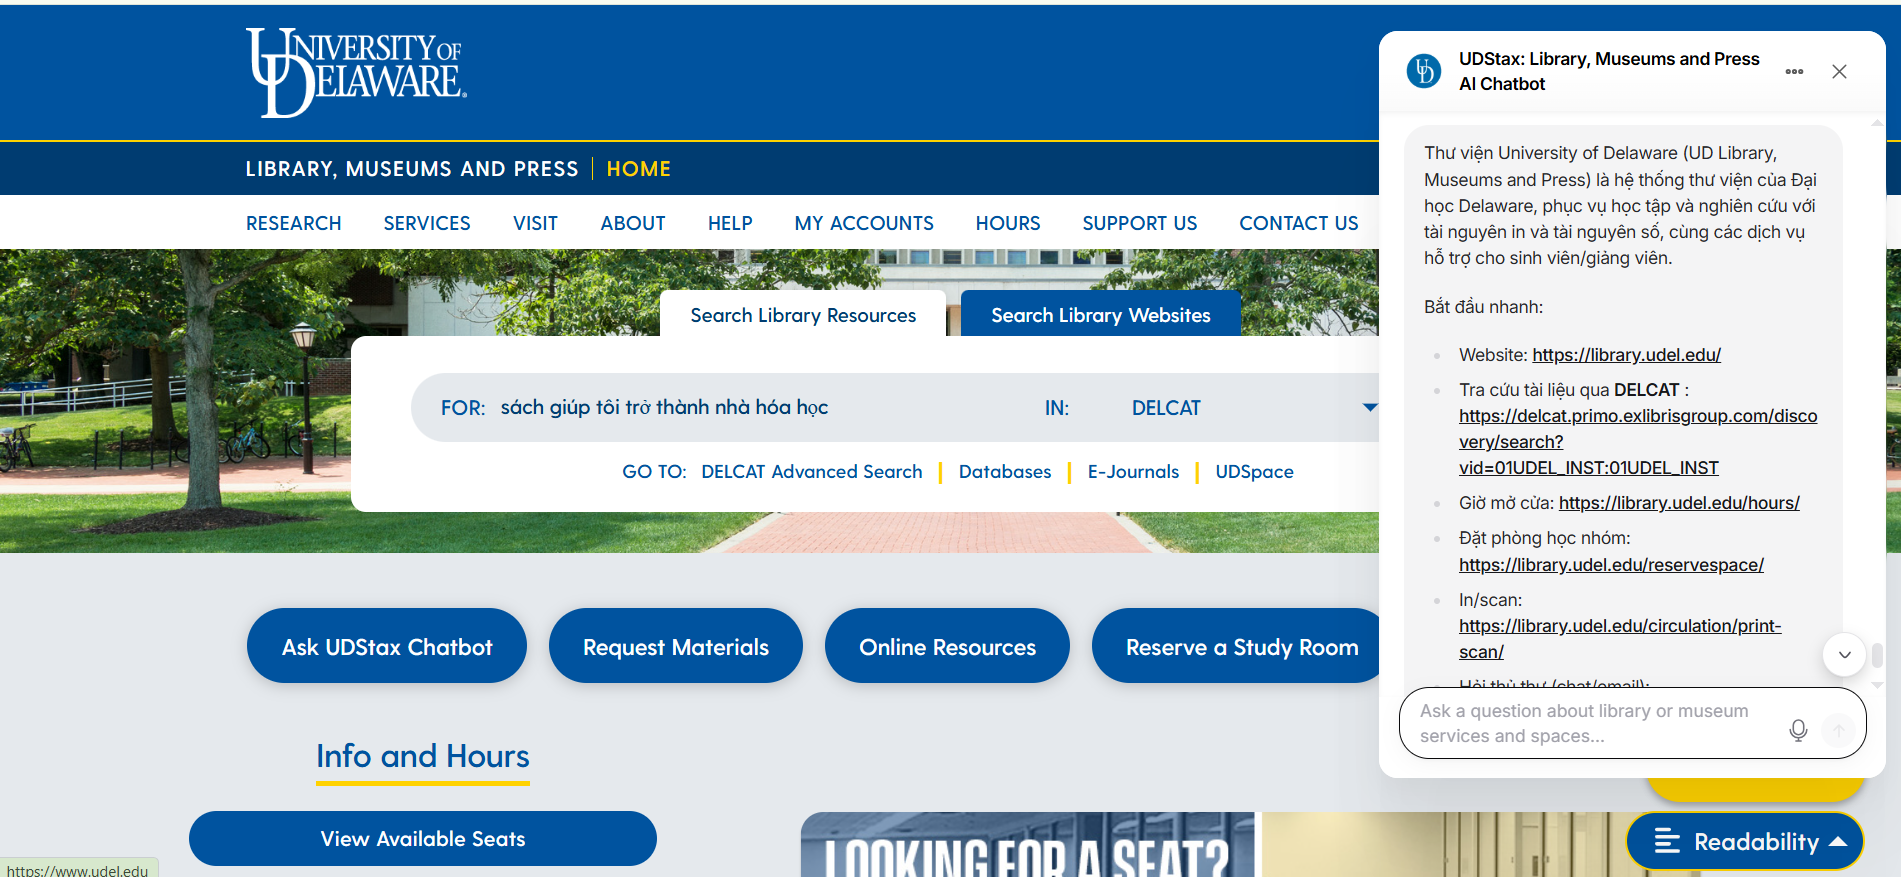
\includegraphics[width=0.8\linewidth]{Images/ud_library_homepage_chatbot.png} 
\vspace{10pt}
\caption{Giao diện dịch vụ khám phá hợp nhất DELCAT và công cụ AI hỗ trợ tại Thư viện UD}
\label{fig:ud_delcat_search}
\end{figure}

Tìm hiểu UD Library mang lại các góc nhìn kiến trúc quan trọng về việc xây dựng một nền tảng khám phá hợp nhất "Tất cả trong một" và vận hành các trợ lý AI giao tiếp trong môi trường học thuật lớn.

\subsubsection{Ưu điểm}
\begin{itemize}
\item Tích hợp các trợ lý ảo có khả năng xử lý ngôn ngữ tự nhiên để tự động hóa các câu hỏi Q\&A thủ tục thường gặp.
\item Nền tảng DELCAT hợp nhất việc khám phá sách in và tài nguyên điện tử trong một giao diện người dùng duy nhất.
\item Kết nối các dịch vụ thư viện phi truyền thống, như đặt phòng học nhóm, dịch vụ in ấn và mượn liên thư viện.
\end{itemize}

\subsubsection{Hạn chế}
\begin{itemize}
\item Chatbot hoạt động độc lập như một kênh tư vấn thủ tục mà chưa tích hợp sâu vào động cơ tìm kiếm để gợi ý sách trực tiếp.
\item Kiến trúc khám phá hợp nhất thường xuyên gây quá tải thông tin bằng cách trả về lượng kết quả tìm kiếm quá lớn.
\end{itemize}

\subsection{Hệ thống Quản lý Thư viện Mã nguồn Mở -- Koha ILS}

Koha ILS là Hệ thống Thư viện Tích hợp (ILS) mã nguồn mở được áp dụng rộng rãi nhất trên thế giới, được sử dụng bởi nhiều định chế giáo dục và mạng lưới thư viện công cộng. Khác với các cổng OPAC dành cho người dùng hoặc các nền tảng Khám phá được phân tích ở trên, Koha đại diện cho một hệ thống lõi backend tập trung vào việc số hóa và tự động hóa các quy trình quản lý hành chính phức tạp cho nhân viên thư viện (Thủ thư).

Thông qua cổng quản trị Staff Client, Koha cung cấp các mô-đun toàn diện để quản lý thư viện vật lý và thư viện số, bao gồm: Lưu thông, Biên mục Quốc tế, Quản lý Độc giả và Báo cáo Thống kê. Việc nghiên cứu Koha cung cấp các tiêu chuẩn tham chiếu giá trị cho việc thiết kế lược đồ cơ sở dữ liệu và logic quy tắc nghiệp vụ trong đồ án của chúng tôi.

\begin{figure}[H]
\centering
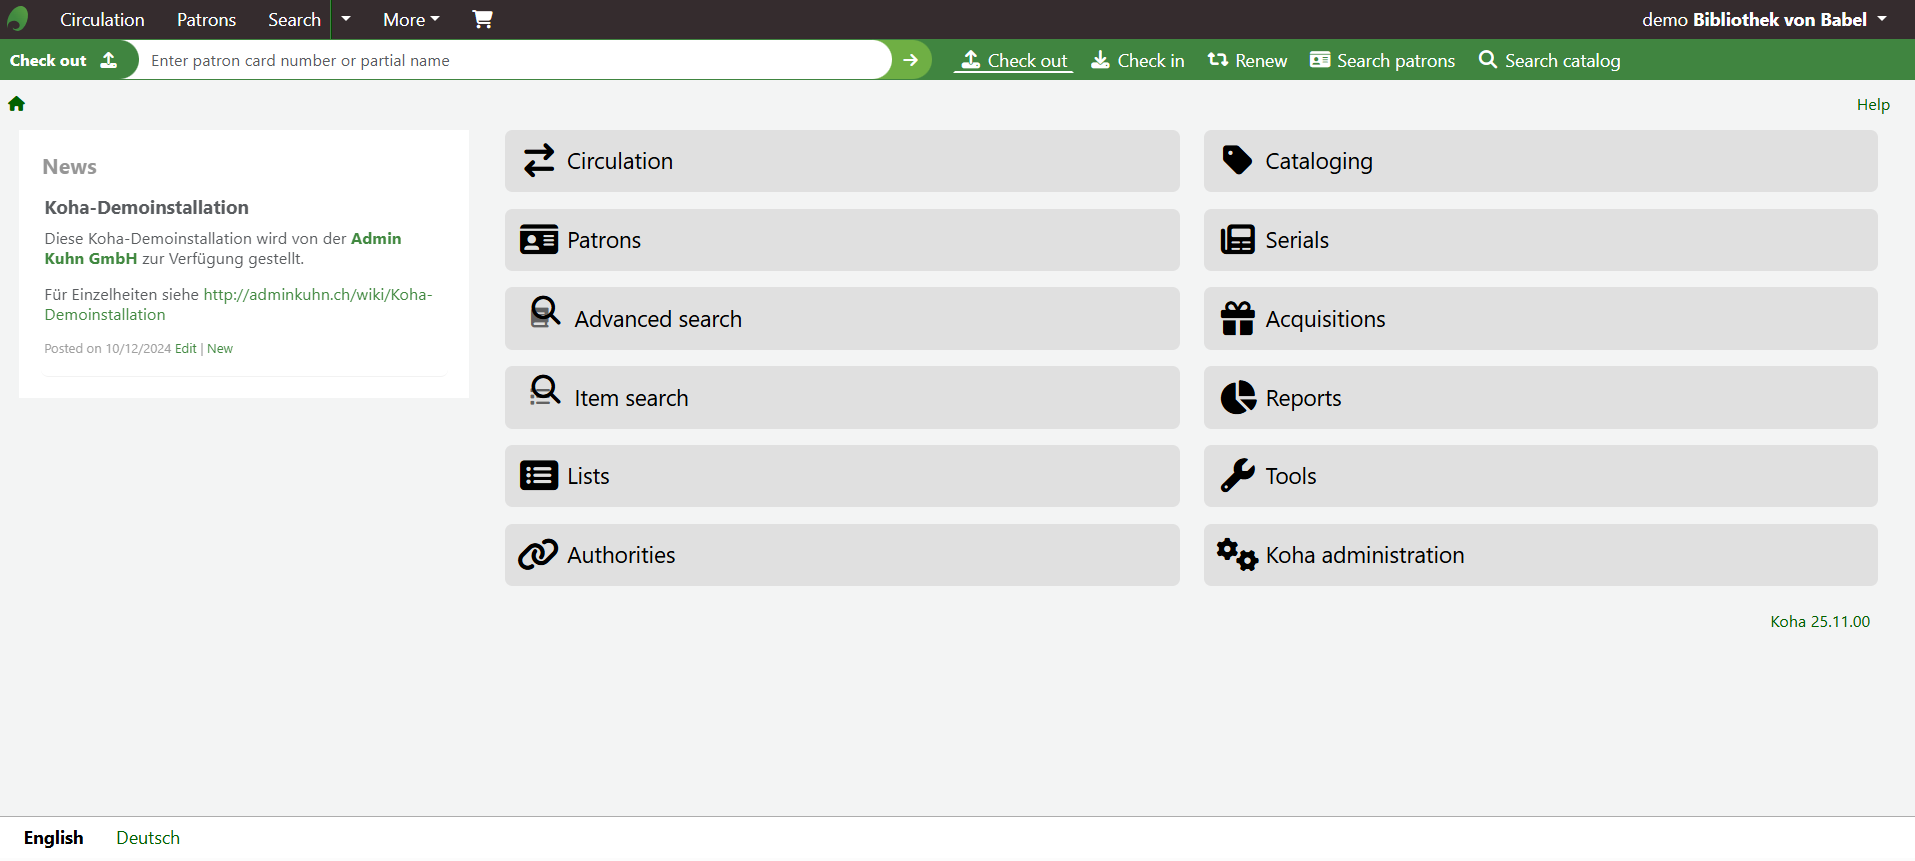
\includegraphics[width=0.8\linewidth]{Images/koha_staff_interface.png} 
\vspace{10pt}
\caption{Mô-đun giao diện quản trị Staff Client của Koha}
\label{fig:koha_admin}
\end{figure}

Phân tích Koha giúp xác định rõ các tính năng cốt lõi cần thiết trong một phần mềm quản lý thư viện, đồng thời chỉ ra các điểm bất tiện trong trải nghiệm người dùng hiện diện ở các hệ thống quản trị truyền thống.

\subsubsection{Ưu điểm}
\begin{itemize}
\item Tuân thủ nghiêm ngặt các tiêu chuẩn dữ liệu tả thư viện quốc tế (MARC21, Z39.50), đảm bảo tính nhất quán và khả năng tương thao dữ liệu.
\item Mô-đun lưu thông cung cấp ma trận quy tắc chi tiết để cấu hình logic mượn, trả, gia hạn và phạt quá hạn phù hợp với từng nhóm người dùng.
\item Tích hợp sẵn các REST API cho phép các ứng dụng bên thứ ba tương tác và trích xuất dữ liệu để mở rộng nền tảng.
\item Hệ thống báo cáo hỗ trợ các truy vấn SQL tùy chỉnh trực tiếp, mang lại sự linh hoạt tối đa cho các báo cáo quản trị.
\end{itemize}

\subsubsection{Hạn chế}
\begin{itemize}
\item Giao diện Staff Client (UI/UX) phức tạp, tuân theo các bố cục nhiều biểu mẫu truyền thống làm tăng thời gian đào tạo thủ thư.
\item Quy trình biên mục dữ liệu vẫn phụ thuộc nặng nề vào thao tác thủ công, thiếu các cơ chế phân loại tự động thông minh hoặc trích xuất dữ liệu tả.
\item Kiến trúc hệ thống đơn khối (monolithic) và lược đồ cơ sở dữ liệu quan hệ phức tạp cản trở việc tách biệt nhanh chóng hoặc bổ sung các tính năng mô-đun tùy chỉnh.
\end{itemize}